
\iffalse
To Do:
Re-write abstract
Re-write methods

In future will rewrite such that KL is obeyed
But as a thought experiment, if the number of samples goes to infinity, shouldn't the distance metric between the datasets generated from the physical process go to 0?


Include XaFai, Phialia's stuff
Need to do a better job of explaining why 5 million datapoints isn’t enough, - •	Compare times between GEMC and NF training
Our physics data is on order 10M events, so we need order 100M events, the optimal single thread processing size is 10k events, which takes 5 hours to process, meaning 100M events will take 50k core hours. However, the distributions are reasonably well defined after processing only a few million event.s 


Add more discussion of relevant work (Stan's work). How is our problem different?

\fi

\begin{abstract}
We demonstrate a proof of principle for using a normalizing flow to learn a physics process's probability distribution to effectively sample more data. In this work, we used traditional physics simulations to generate a dataset $\mathbf{x}$ has 5 million data points of 4 features. We take as input $p(\mathbf{z})$ a constant 4D normal distribution, and examine whether the flow model can learn the transformation to $p(\mathbf{x})$. We observed a reasonable agreement between the given physics sample and the newly-sampled data using the flow model both in visualization and quantified the metrics.
\end{abstract}
\section{Introduction including Related Works }
%(we can now cite Stan's work! \textcolor{red}{did he already submit his thesis to DSpace MIT?})

Large scale particle physics experiments use humankind's largest machines to study nature at the smallest scales. One such experiment, called CLAS12 in Virginia at the Thomas Jefferson National Accelerator Facility (JLab) (\citet{BURKERT2020163419}), collides ultrarelativistic electrons moving only 1 m/s slower than the speed of light into an ultracold bunch of hydrogen to glean information about the substructure of the proton. In particular, two photons, one electron and one proton in the final state is known as Deeply Virtual $\pi^0$ Production (DV$\pi^0$P), and this process is currently under detailed study as its properties are related to the mechanical properties of the proton (\citet{PhysRevD.55.7114}).

Typically, real data is compared with the output of detailed simulations of the experiment, wherein Monte-Carlo (MC) methods are used to walk simulated particles through a detector system in many small time steps (\citet{PhysRevLett.115.212003, 10.1093/ptep/ptaa104}). The standard simulation consists of two steps. First, we generate a data set of particle features - momenta and other properties - based on a combination of field-theoretic functions and empirical physics models, which creates an `event' of a realistic four-particle final state from the DV$\pi^0$P process. This generation is very simple and computationally inexpensive. The second step is, for each event, walk all four particles through the simulated detector setup using the GEANT4 package (\citet{AGOSTINELLI2003250}). The output from this step is our four particles that we began with, but with their features smeared out. This second step is the one we are trying to supplement, as it would take about 5,000 hours on a single core machine to process 1 million events. However, through HPCC we have produced so far 100 M generated (step 1) and simulated (step 2) events that can be used for algorithmic training. 

The normalizing flow is an effective model to learn a probability distribution $p(x)$ when a sample data set $X=\{x\}$ following the distribution is given. The basic idea is a series of transformation $g_i$'s, which are referred to as flows, transforms a prior probability $p(z)$ distributions into the target distribution $p(x)$. That is
\begin{align}
    \mathbf{x} =& g_N \circ g_{N-1}\circ ... \circ g_1 (\mathbf{z}) \\
    \mathbf{z} =& f_1 \circ ... \circ f_{N-1} \circ f_N (\mathbf{x}) \label{eqn:invertible}
\end{align}
, where $f_{N-i+1}\equiv g_i^{-1}$ following \citet{9089305}'s convention. Both $\mathbf{x}$ and $\mathbf{z}$ are vectors of the same dimension $d$. From the eq.~\ref{eqn:invertible}, $g_i$ requires an invertibility condition. An intermediate flow $\mathbf{z_i}$ is defined as follows.
\begin{align}
\mathbf{z_i} =&g_i \circ ... \circ g_1(\mathbf{z}) \label{eqn:forward}\\
    =&f_{i+1}\circ ...f_N(\mathbf{x}) \label{eqn:backward}
\end{align}
, where the flow is expressed in forward direction at eq.~\ref{eqn:forward}, and in backward direction at eq.~\ref{eqn:backward}. Therefore, $\mathbf{z_{i+1}}=g_i (\mathbf{z_i})$ and $\mathbf{z_i} = f_{N-i+1}(\mathbf{z_{i+1}})$ for one flow, or layer. If the $f_i$'s are differentiable, the PDF evolves as follows.
\begin{align}
 p(\mathbf{z_{i+1}})=& p(\mathbf{z_i})|\frac{\partial f_{N-i+1}}{\partial \mathbf{z_i}}| =p(\mathbf{z_i})|\frac{\partial g_{i}^{-1}}{\partial \mathbf{z_i}}|\\
 \log p(\mathbf{z_{i+1}}) =& \log p(\mathbf{z_i}) + \log|\frac{\partial g_i^{-1}}{\partial \mathbf{z_i}}| \label{eqn:logprob}\\
 \log p(\mathbf{x}) =& \log p(\mathbf{z}) + \sum\limits_{i=1}^N \log|\frac{\partial g_i^{-1}}{\partial \mathbf{z_i}}|.
\end{align}
Eq.~\ref{eqn:logprob} is useful to define the forward and the backward propagation of each layer.
Once the NF model is trained to learn the distribution $g: p(z)\rightarrow p(x)$, it is possible to sample $x$ using sampled $z$. \citet{PhysRevD.101.076002} showed that the Nonlinear Independent Component Estimation (NICE) (\citet{Dinh15}) implementation of NF performs well by comparing the technique to existing methods in terms of efficiencies that are defined as average weight during the generation.

Motivated by \citet{stan}'s work, we use Masked Autoregressive Flows (MAF, \citet{papamakarios2018masked}), which is one of the generalized versions of NICE. The MAF starts from a simple fact that $p(z_{i}) = \prod\limits_{j}p(z_{i,j}|\mathbf{z}_{i,0:j-1})$. The component $z_{i,j}$ is the $j$-th component of $z_i$, and the vector $\mathbf{z}_{i,0:j-1}$ is defined as $\{z_{i, 0}, ..., z_{i, j-1}\}$. The transformation is finally defined as
\begin{align}
    z_{i+1, j}=& \sigma_{i, j} z_{i, j} + \mu_{i+1, j}.
\end{align}
The moments $\mu_{i+1, j}$ and $\sigma_{i, j}$ are the mean and standard deviation of $p(z_{i+1,j}|\mathbf{z}_{i+1,0:j-1})$ ($\equiv p(z_{i+1,0})$ for $j=0$). We train the flows to learn $\mu_{i+1, j}$'s and $\sigma_{i, j}$'s, and sample $p(\mathbf{x})$.

\citet{papamakarios2018masked} presents a good github repository of how to train a NF for a 2-dimensional distribution. The libraries are very straightforward and use PyTorch. The architecture consists of the two layers of MAF and the 2D normal prior distribution.

\section{Methods}
%We should include our work of generating the data (GEMC) and processing the data (convert to root, pandas, pickle) as these are all non-trivial steps and a good "data pipeline"
The data of 5M `events`, or sets of data points, in this problem has been achieved from Open Science Grid (OSG). The original data format is in ROOT \cite{root}, which is a widely-used format in high energy physics written in C++. There have been improvements in python libraries like uproot \cite{uproot} that can interpret the ROOT data format. The data file has been read using uproot, and saved in pickle, a standard Python library for serializing data \footnote{\url{https://github.com/6862-2021SP-team3/hipo2pickle}}. The pickled data has 5M row, each of which contains the features of four individual particles. Each individual particle has 3 features (magnitude of momentum, polar angle, azimuthal angle), but for the milestone report, we have tried with only the magnitude of momenta of all four particles. So our sample $\mathbf{x}$ has dimensions of $5\text{M}\times4$. The sampled $\mathbf{z}$ has the same dimensions, but as sampled data points, not in the analytic distributions.  We expect to learn the distribution of sample $\mathbf{z}$'s with another NF, and use that distribution of prior in the final results. But we ignore the actual $\mathbf{z}$ distributions, and try with the constant distributions at this stage.

We forked the repository in our organizaztion, and applied the libraries for our purpose\footnote{\url{https://github.com/6862-2021SP-team3/nflows/blob/master/nflow.ipynb}}. We have 10 layers of MAF. We have 1k training steps, each of which consists of randomly sampled training data sets of $1\text{k}\times$4 dimension. To evaluate, we randomly take 100k$\times$4 data points $\mathbf{x_1}$ from 5M data points, and sample another set of 100k$\times$4 data points, $\mathbf{x_2}$, using the trained MAF. We checked the three metrics between $\mathbf{x_1}$ and $\mathbf{x_2}$ , the KL Divergence (KLD, \citet{Kullback51klDivergence}), the Earth Mover's Distance (EMD), also known as the Wasserstein Distance (\citet{Dobrushin}).
%the Jensen-Shannon divergence (JSD, \citet{jsd}).

\section{Preliminary Results}
Fig.~\ref{fig:a} visualizes the 2D distributions of the test data $\mathbf{x_1}$ and $\mathbf{x_2}$. We mean 2D distributions of features 0 and 1 by the EP distribution and features 2 and 3 by the GG distribution. We also draw 1D distributions of each feature in Fig.~\ref{fig:b}'s top row. To directly compare, another set of 100k$\times$4 data points, $\mathbf{x_3}$ is sampled in the bottom of Fig.~\ref{fig:b}. Qualitatively, the MAF generated data generally follows the microphysics generated data, but differ in detailed shape. At this stage it is not clear what is causing this discrepancy, or how it can be mitigated. It is possible that including more features in training will provide higher fidelity results due to the correlations between features, but this is an active area of our research.

\begin{figure}[!ht]
    \centering
    \begin{minipage}{.4\textwidth}
    Feature Distribution: Physics Data
        \centering
        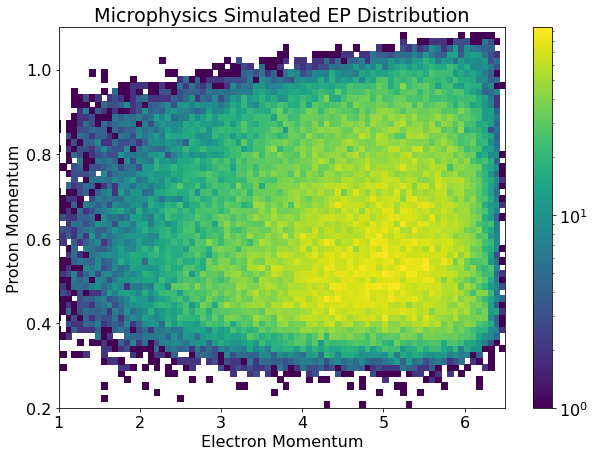
\includegraphics[width=.9\textwidth,trim={0 0 0 0},clip]{pictures/milestoneR2/gemc1.png}
        %\caption{(a)}
        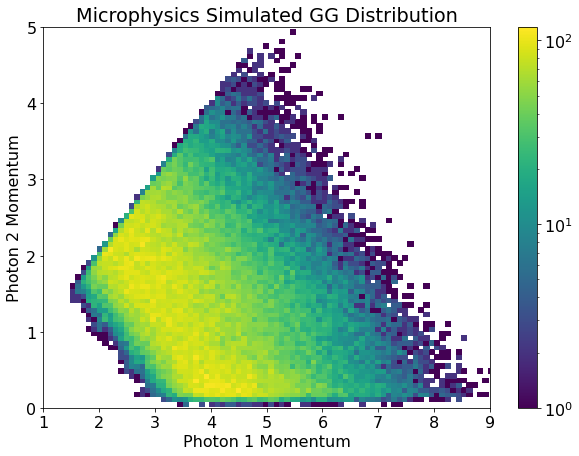
\includegraphics[width=.9\textwidth,trim={0 0 0 0},clip]{pictures/milestoneR2/gemc2.png}
        %\caption{(c)}
    \end{minipage}%
    \begin{minipage}{0.4\textwidth}
    Feature Distribution: NFlow Generated
        \centering
        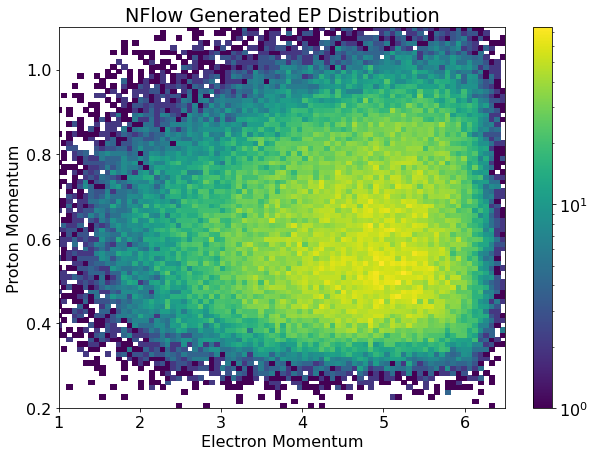
\includegraphics[width=.9\textwidth,trim={0 0 0 0},clip]{pictures/milestoneR2/nflow1.png}
        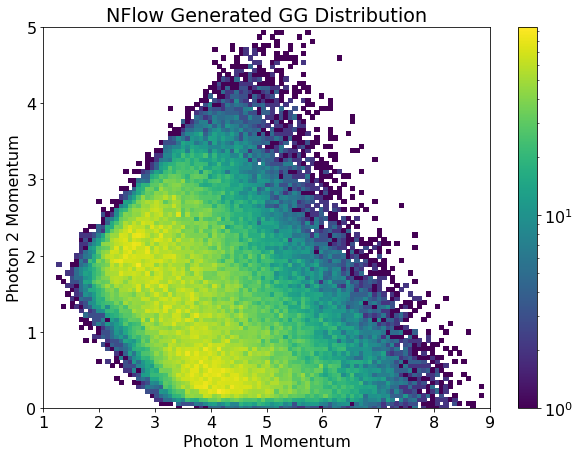
\includegraphics[width=.9\textwidth,trim={0 0 0 0},clip]{pictures/milestoneR2/nflow2.png}
    \end{minipage}
    \caption{Left: the 2D distributions of feature 0 vs. feature 1 (top) and of feature 2 vs. feature 3 (bottom) in $\mathbf{x_1}$. Right: the 2d distributions of feature 0 vs. feature 1 (top) and of feature 2 vs. feature 3 (bottom) in $\mathbf{x_2}$.}
    \label{fig:a}
\end{figure}

\begin{figure}[!ht]
    \centering
    \begin{minipage}{1\textwidth}
    Feature Distribution: Physics Data
        \centering
        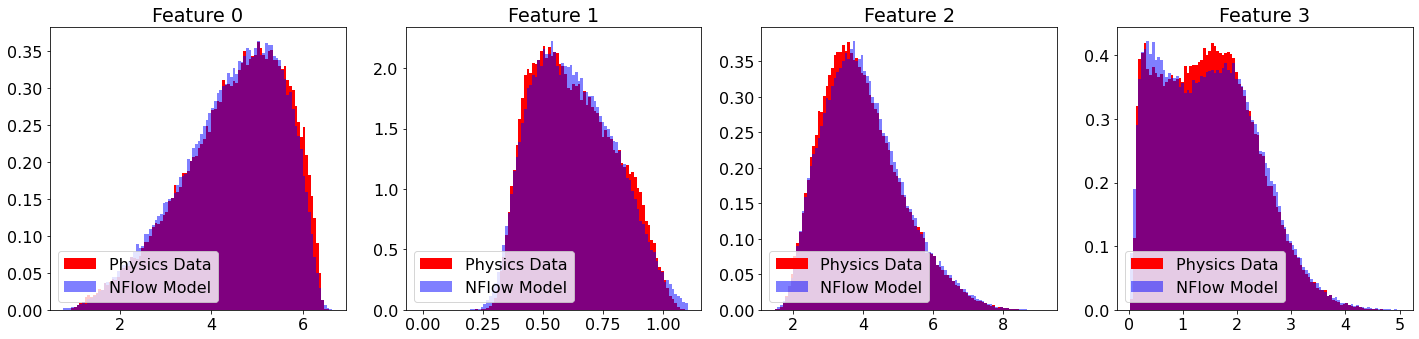
\includegraphics[width=.9\textwidth,trim={0 0 0 0},clip]{pictures/milestoneR2/comp1.png}
        %\caption{(a)}
        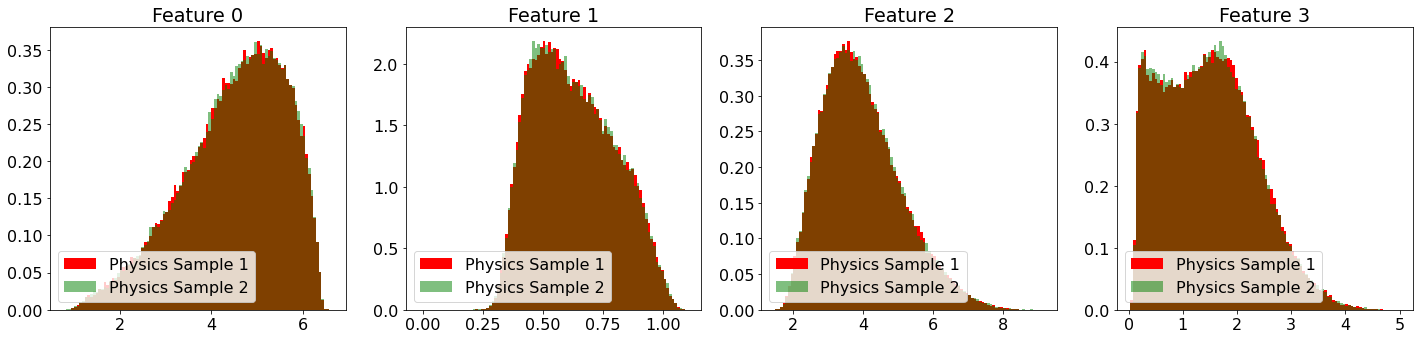
\includegraphics[width=.9\textwidth,trim={0 0 0 0},clip]{pictures/milestoneR2/comp2.png}
        %\caption{(c)}
    \end{minipage}%
    \caption{Top: four plots visualizing 1D distributions of each feature in $\mathbf{x_1}$ (labeled as `Physics Data') and $\mathbf{x_2}$ (labeled as `NFlow Model'). Bottom: four plots visualizing 1D distributions of each feature in $\mathbf{x_1}$ (labeled as `Physics Sample 1') and $\mathbf{x_3}$ (labeled as `Physics Sample 2').}
    \label{fig:b}
\end{figure}


\begin{center}
\begin{tabular}{ |p{2.5cm}||p{1.4cm}|p{1.4cm}|p{1.4cm} |p{1.4cm}| }
 \hline
 \multicolumn{5}{|c|}{Values of EMD and KLD for Fig.~\ref{fig:b}} \\ 
 \hline
%Quantity &  \multicolumn{4}{|c|}{Feature Number} \\ 
\textbf{Quantity} & \textbf{Feature 0} & \textbf{Feature 1} & \textbf{Feature 2} & \textbf{Feature 3} \\
 \hline                                             
%\multirow{2}{4em}{EMD}  & 0.0671 & 0.0048 & 0.0469 & 0.03533\\ 
EMD - NFlow  & 0.0671 & 0.0048 & 0.0469 & 0.0353\\ 
EMD - Sample & 0.0111 & 0.0006 & 0.0148 & 0.0038\\ 

\hhline{|=|=|=|=|=|}
%\multirow{2}{4em}{KLD} & $\infty$ & 0.0748 & 0.07969 & $\infty$\\ 
KLD- NFlow & $\infty$ & 0.0748 & 0.07969 & $\infty$\\ 
KLD - Sample & 0.0721 & 0.0730 & 0.07962 & 0.3973 \\ 

 \hline
\end{tabular}
\end{center}

\iffalse
\begin{center}
\begin{tabular}{c c c c c c }
Quantity & F0 & F1 & F2 & F3  \\
\hline
NFlow EMD & 0.0671 & 0.0048 & 0.0469 & 0.0353 \\ 
Sample EMD & 0.0111 & 0.0006 & 0.0148 & 0.0038 \\
NFlow KLD & $\infty$ & 0.0748 & 0.07969 & $\infty$\\  
Sample KLD & 0.0721 & 0.0730 & 0.07962 & 0.3973\\ 
\end{tabular}
\end{center}
\fi

The right subplot of Fig.~\ref{fig:c} shows the EMD vs. iteration in training, from which we can see that after about 1,000 steps we converge to a minimum loss value. We presented the progress of NF training results compared to the physics distributions at the left of Fig.~\ref{fig:c}.


\begin{figure}[!ht]
    \centering
    \begin{minipage}{.25\textwidth}
    
        \centering
        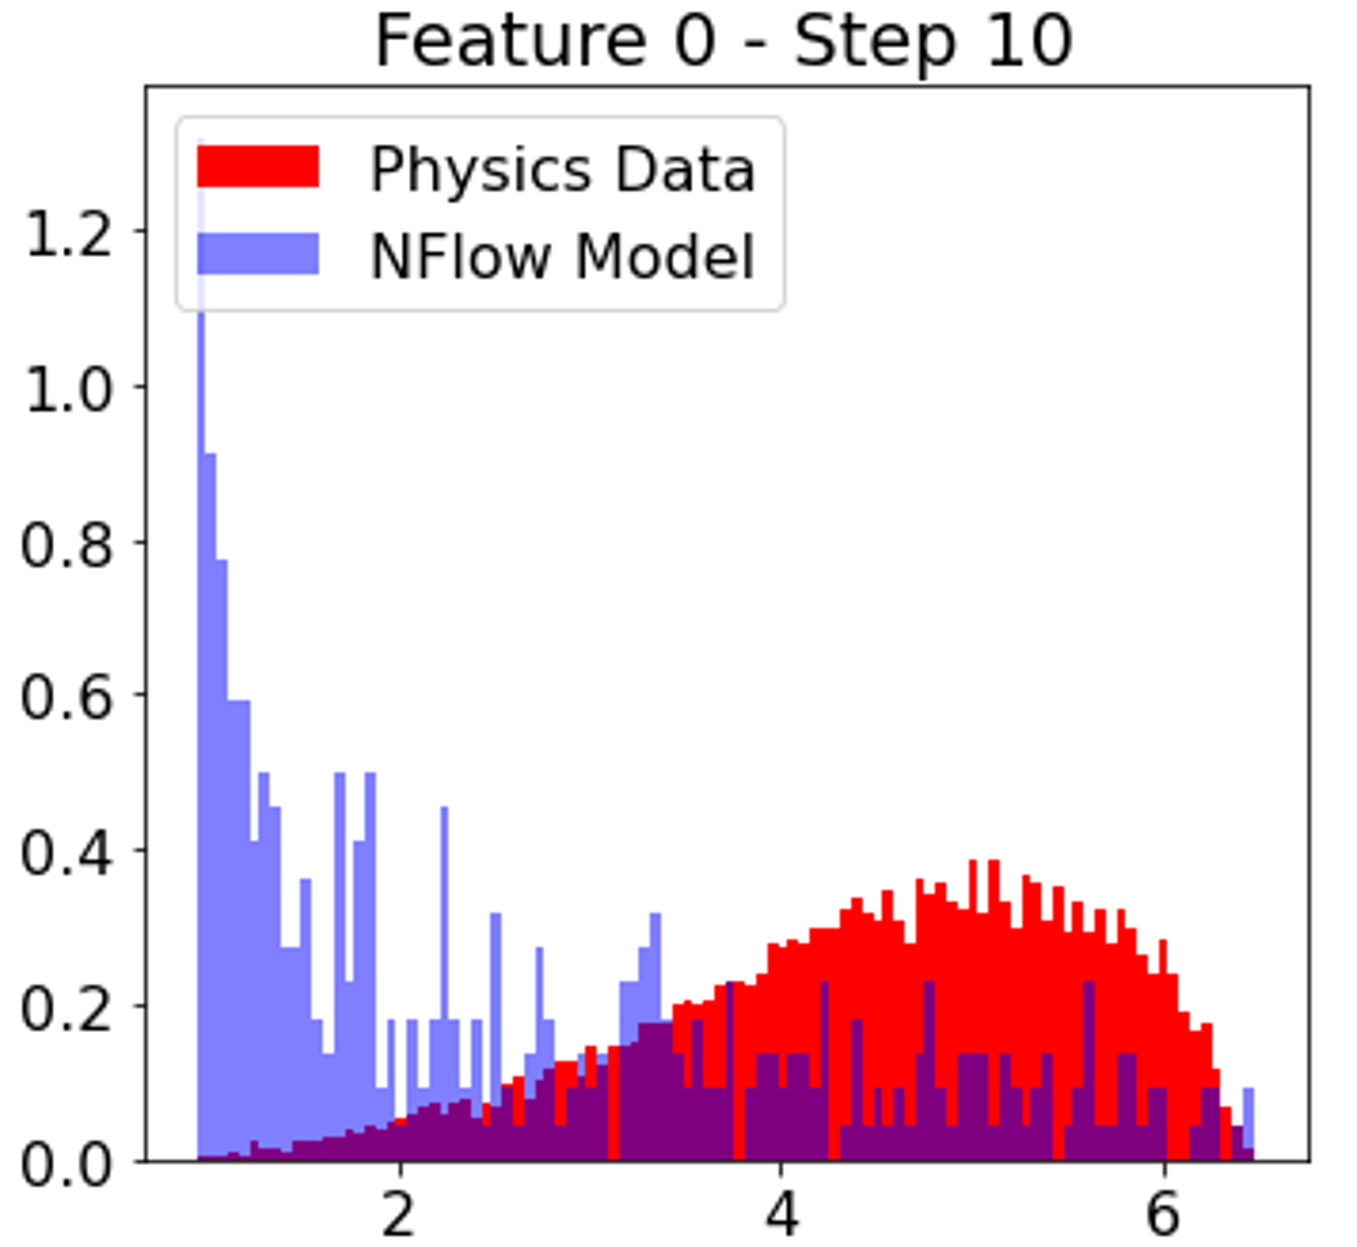
\includegraphics[width=.9\textwidth,trim={0 0 0 0},clip]{pictures/milestoneR2/steps/s10.png}
        %\caption{(a)}
        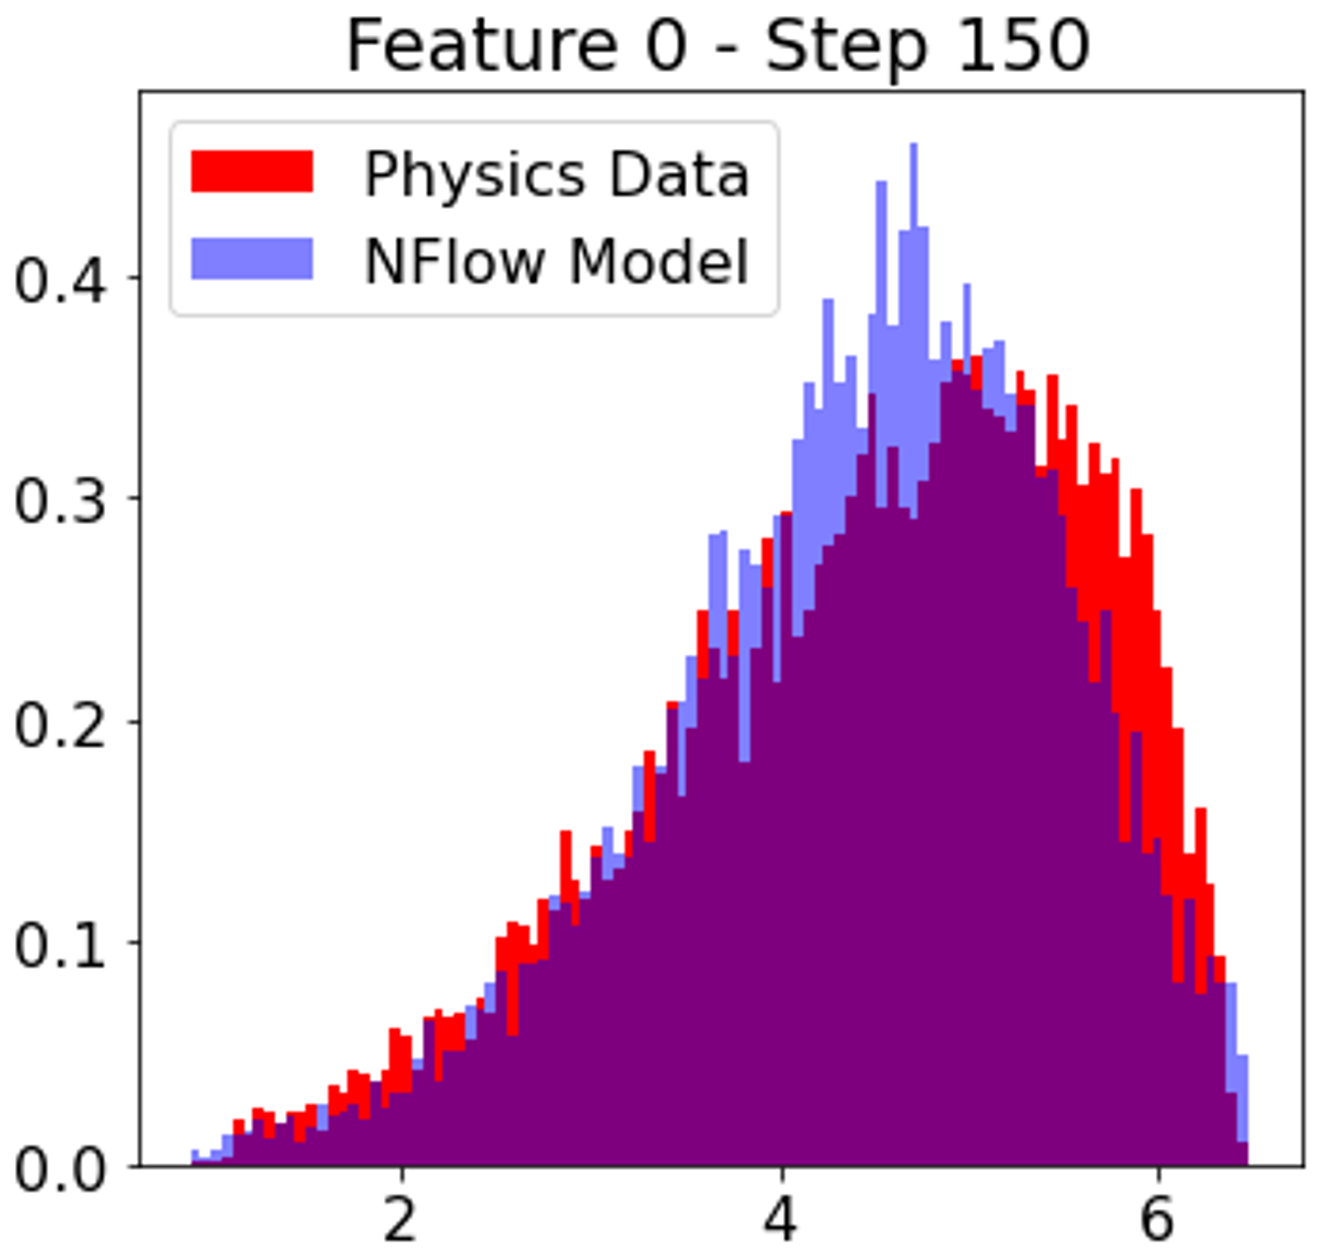
\includegraphics[width=.9\textwidth,trim={0 0 0 0},clip]{pictures/milestoneR2/steps/s150.png}
        %\caption{(c)}
    \end{minipage}%
    \begin{minipage}{0.25\textwidth}
    
        \centering
        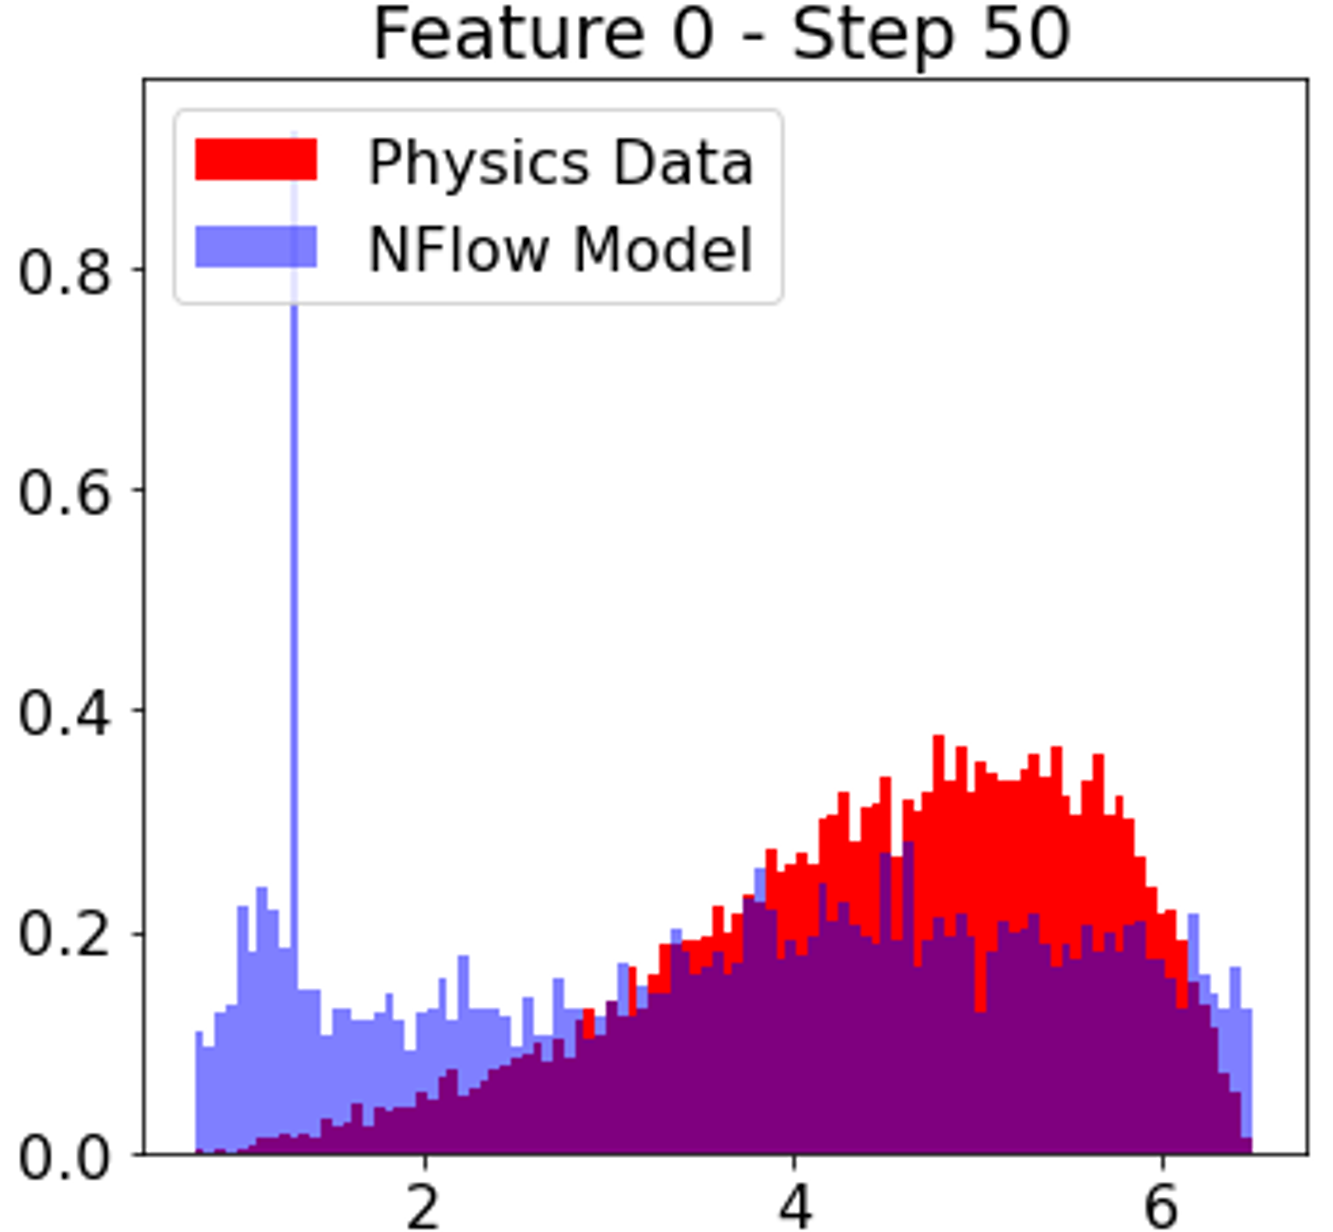
\includegraphics[width=.9\textwidth,trim={0 0 0 0},clip]{pictures/milestoneR2/steps/s50.png}
        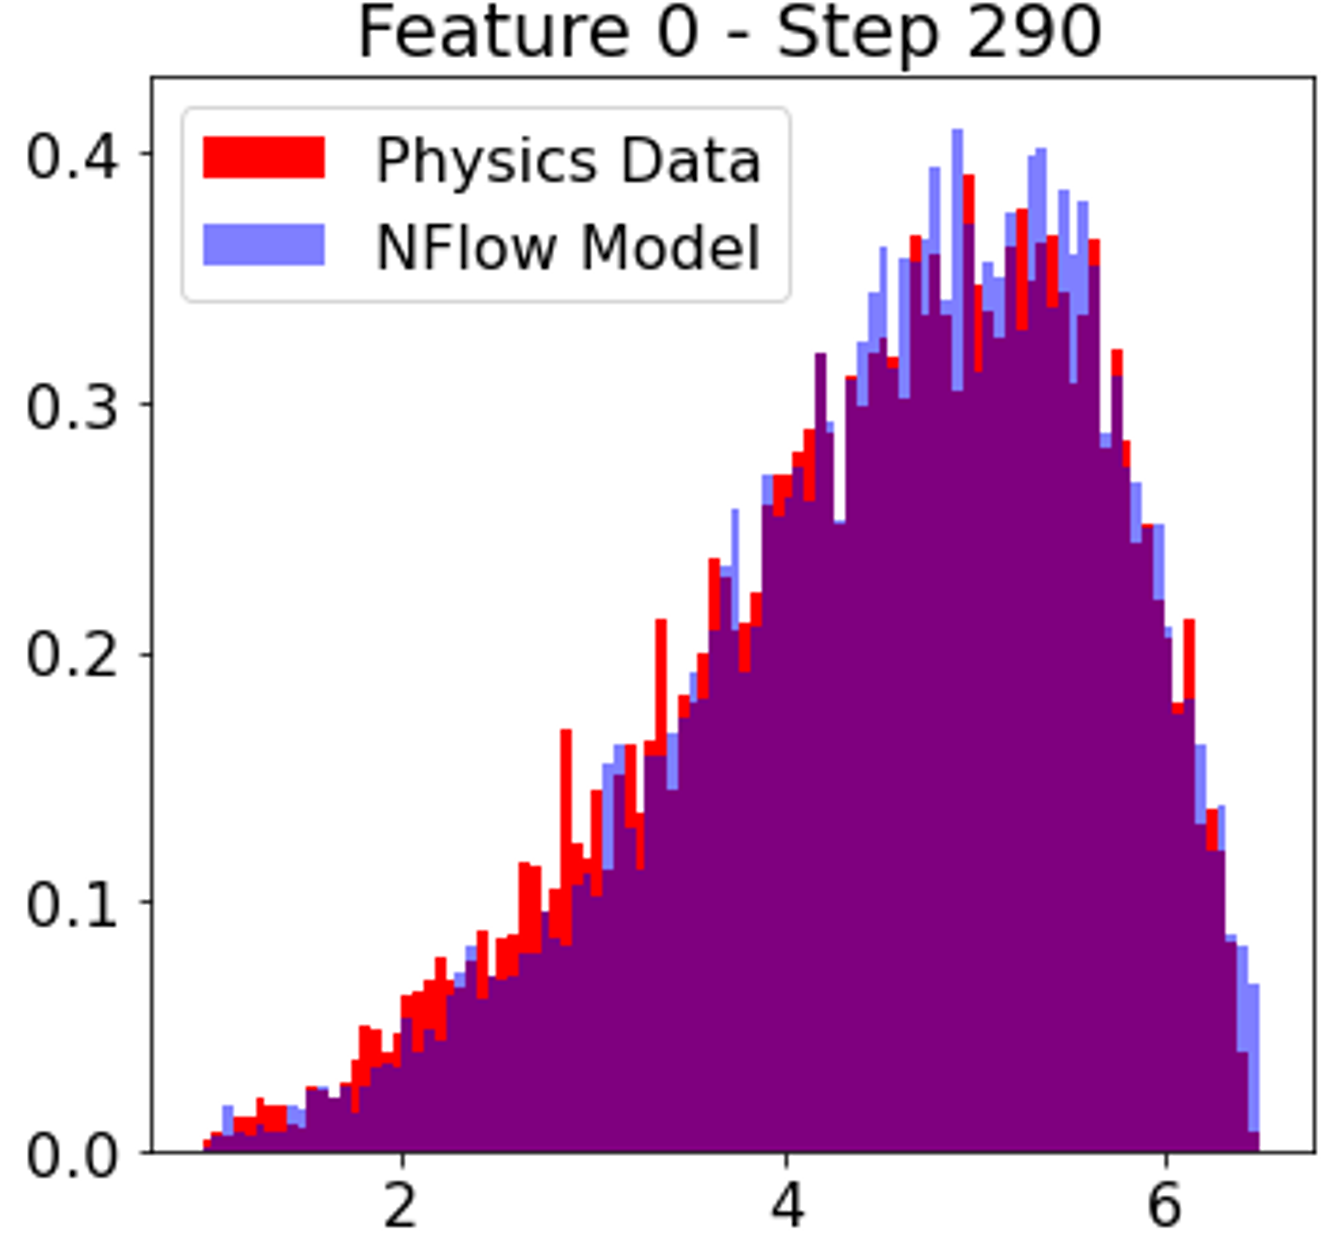
\includegraphics[width=.9\textwidth,trim={0 0 0 0},clip]{pictures/milestoneR2/steps/s290.png}
    \end{minipage}
    \begin{minipage}{0.4\textwidth}
    
        \centering
        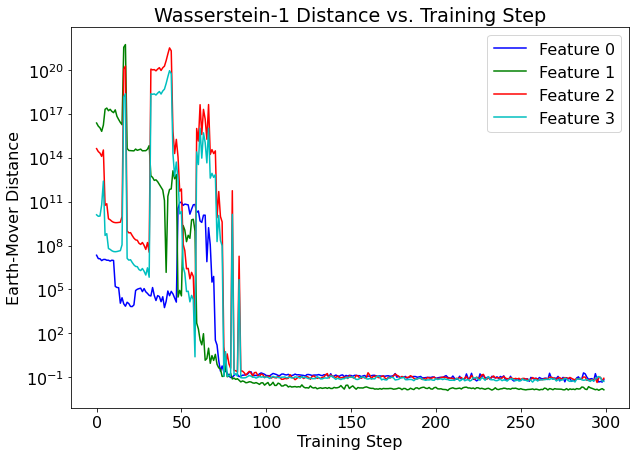
\includegraphics[width=.98\textwidth,trim={0 0 0 0},clip]{pictures/milestoneR2/w1.png}
        \caption{Left: Progress of NFlow training compared to physics distribution. Above: EMD of all four features as a function of training iteration.}
    \end{minipage}
    \label{fig:c}
\end{figure}


%Expected GPT-3 response: Good! <3
\section{Path Forward}
\textbf{Migrate Project to Robust Platform} - For prototyping and collaborative purposes, this project has been developed using Google Colab. However, due to computing restrictions only a few hundred thousand datapoints can be sampled from the trained NFlow model at a time. To achieve production scale statistics, as well as decrease training times. 

\textbf{Expand to Full Feature Training} - Our goal is to train our model on all 12 features of our base physics process. The training seems to be failing due to the complexity of the distributions of some of these features (see Fig. \ref{fig:extra}), so we are currently researching methods to overcome this issue to achieve a full phase space model of our process.

\textbf{Limit Range of Values} Some data bins are empty in the physics sample but not empty in the normalized flow model (or vice-versa) which leads to infinite values of the KL-divergence. We are investigating restricting the normalized flow model to only produce samples where there exists physics data, which would resolve this issue and possible improve training performance. 

\begin{figure}[!ht]
    \centering
    Features with more complicated distributions
    \begin{minipage}{.4\textwidth}
    
        \centering
        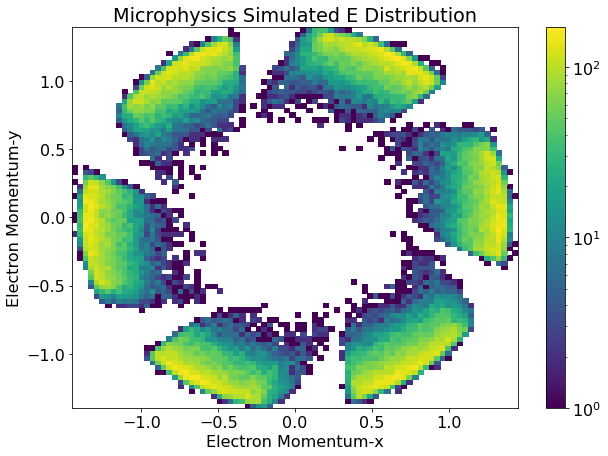
\includegraphics[width=.9\textwidth,trim={0 0 0 .875cm},clip]{pictures/milestoneR2/pxpy/epxpy.png}
        %\caption{(a)}
        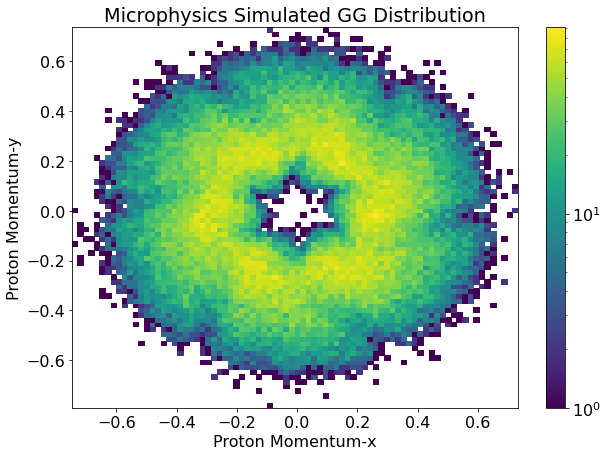
\includegraphics[width=.9\textwidth,trim={0 0 0 .875cm},clip]{pictures/milestoneR2/pxpy/ppxpy.png}
        %\caption{(c)}
    \end{minipage}%
    \begin{minipage}{0.4\textwidth}
    
        \centering
        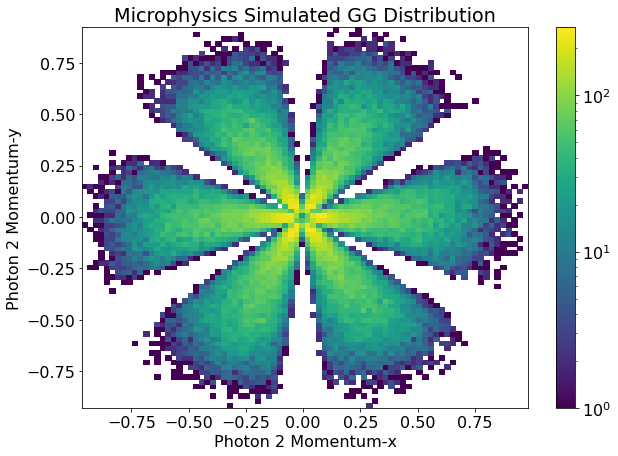
\includegraphics[width=.9\textwidth,trim={0 0 0 .875cm},clip]{pictures/milestoneR2/pxpy/g2pxpy.png}
        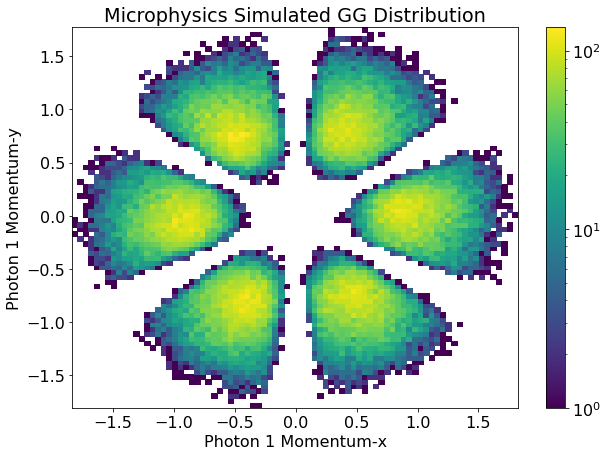
\includegraphics[width=.9\textwidth,trim={0 0 0 .875cm},clip]{pictures/milestoneR2/pxpy/gpxpy.png}
    \end{minipage}
    \caption{Nontrivial feature distributions from physics data that are yet to be modeled successfully by the NFlow model.}
    \label{fig:extra}
\end{figure}


\iffalse
Path forward:\\
Utilization of "z" distribution to train prior distribution\\
Expand to full feature representation learning\\
\fi


\iffalse
Parameters for best run:

prior = TransformedDistribution(Uniform(torch.zeros(2), torch.ones(2)), SigmoidTransform().inv) # Logistic distribution
#prior = MultivariateNormal(torch.zeros(2), torch.eye(2))
# NICE
flows = [AffineHalfFlow(dim=2, parity=i%2, scale=False) for i in range(12)]
#print(flows)
flows.append(AffineConstantFlow(dim=2, shift=False))
#print(flows)


# construct the model
model = NormalizingFlowModel(prior, flows)

optimizer = optim.Adam(model.parameters(), lr=5e-4, weight\_decay=1e-9)
for k in range(5000):
    sampleDict = xz.sample(1000)
    

 Path forward:
 working just on google colab, we quickly run into computing performance issues
 \fi